% !TeX spellcheck = en_US
\documentclass[10pt,a4paper,twocolumn,twoside]{article}
\usepackage[utf8]{inputenc}
\usepackage[english]{babel}
\usepackage{multicol}
\usepackage{graphicx}
\usepackage{fancyhdr}
\usepackage{times}
\usepackage{titlesec}
\usepackage{multirow}
\usepackage{lettrine}
\usepackage{pdflscape}
\usepackage{subcaption}
\usepackage{booktabs}
\usepackage[table,xcdraw]{xcolor}
\usepackage[edges]{forest}
\usepackage{url}
\usepackage[top=2cm, bottom=1.5cm, left=2cm, right=2cm]{geometry}
\usepackage[figurename=Fig.,tablename=Table]{caption}

\author{\LARGE\sffamily Segovia Barreales, Richard}
\title{\Huge{\sffamily Reducing dizziness when using a video-see-through head-mounted display}}
\date{}

\newcommand\blfootnote[1]{%
  \begingroup
  \renewcommand\thefootnote{}\footnote{#1}%
  \addtocounter{footnote}{-1}%
  \endgroup
}

%
%\large\bfseries\sffamily
\titleformat{\section}
{\large\sffamily\scshape\bfseries}
{\textbf{\thesection}}{1em}{}

\begin{document}

	\fancyhead[LO]{\scriptsize AUTHOR: SEGOVIA BARREALES, RICHARD}
	\fancyhead[RO]{\thepage}
	\fancyhead[LE]{\thepage}
	\fancyhead[RE]{\scriptsize EE/UAB TFG INFORMÀTICA: REDUCING DIZZINESS WHEN USING A VIDEO-SEE-THROUGH HEAD-MOUNTED DISPLAY}
	
	\fancyfoot[CO,CE]{}
	
	\fancypagestyle{primerapagina}
	{
	   \fancyhf{}
	   \fancyhead[L]{\scriptsize TFG EN ENGINYERIA INFORMÀTICA, ESCOLA D'ENGINYERIA (EE), UNIVERSITAT AUTÒNOMA DE BARCELONA (UAB)}
	   \fancyfoot[C]{\scriptsize June 2018, Escola d'Enginyeria (UAB)}
	}
	
	%\lhead{\thepage}
	%\chead{}
	%\rhead{\tiny EE/UAB TFG INFORMÀTICA: TÍTOL (ABREUJAT SI ÉS MOLT LLARG)}
	%\lhead{ EE/UAB \thepage}
	%\lfoot{}
	%\cfoot{\tiny{February 2015, Escola d'Enginyeria (UAB)}}
	%\rfoot{}
	\renewcommand{\headrulewidth}{0pt}
	\renewcommand{\footrulewidth}{0pt}
	\pagestyle{fancy}
	
	%\thispagestyle{myheadings}
	\twocolumn[\begin{@twocolumnfalse}
	
	%\vspace*{-1cm}{\scriptsize TFG EN ENGINYERIA INFORMÀTICA, ESCOLA D'ENGINYERIA (EE), UNIVERSITAT AUTÒNOMA DE BARCELONA (UAB)}
	
	\maketitle
	
	\thispagestyle{primerapagina}
	%\twocolumn[\begin{@twocolumnfalse}
	%\maketitle
	%\begin{abstract}
	\begin{center}
	\parbox{0.915\textwidth}
	{\sffamily
	\textbf{Resum--}
	Els darrers anys, els dispositius de realitat virtual i realitat augmentada són objecte de grans avenços. Tot i això, els usuaris encara pateixen molèsties quan les utilitzen. A les sessions de testeig amb usuaris, s'ha pogut observar que aquests es senten més còmodes quan s'utilitza una configuració de visualització especifica per a cada distància. Utilitzant un generador de mapes de profunditat s'ha implementat un sistema que modifica dinàmicament la configuració de l'usuari segons la distància dels objectes que s'està mirant. Utilitzant aquest sistema, els usuaris han percebut una millora en l'experiència i menys fatiga visual.
	\\
	\\
	\textbf{Paraules clau-- } Acomodació i vergència, mapes de profunditat, calibratge estèreo, visió per computador.\\
	\\
	%\end{abstract}
	%\bigskip
	%\begin{abstract}
	\bigskip
	\\
	\textbf{Abstract--} In the recent years head mounted displays have been a great focus of attention for research development and consumer oriented products. Nevertheless, users still experience dizziness when using them. We observed, in a user testing session, that in video-see-through devices the user experience improves when using different settings for each viewed distance. By using a depth map generator, we implemented a dynamic system that changes the setting depending on the viewed distance, and in another user testing session, users agreed that this system improves their user experience and reduces dizziness. 
	\\
	\\
	\textbf{Keywords-- } Accomodation vergence conflict, video-see-through, head mounted display, depth map, stereo calibration,  computer vision. 
	}
	
	\bigskip
	
	{\vrule depth 0pt height 0.5pt width 4cm\hspace{7.5pt}%
	\raisebox{-3.5pt}{\fontfamily{pzd}\fontencoding{U}\fontseries{m}\fontshape{n}\fontsize{11}{12}\selectfont\char70}%
	\hspace{7.5pt}\vrule depth 0pt height 0.5pt width 4cm\relax}
	
	\end{center}
	
	\bigskip
	%\end{abstract}
	\end{@twocolumnfalse}]
	
	\blfootnote{$\bullet$ E-mail: richard.segovia@e-campus.uab.cat}
	\blfootnote{$\bullet$ Menció en Computació}
	\blfootnote{$\bullet$ Project supervised by: Coen Antens (CVC) and Felipe Lumbreras (Computació)}
	\blfootnote{$\bullet$ Course 2017/18}
	
	\section{Introduction}
	%- introduccion al vr
	%- explicar motivacion, practicas de verano, procarelight, usuarios mareados
	%- explicar projecto en si, idea
	%- explicar Accomodation vergence con un dibujo y de forma resumida
	
	\lettrine[lines=3]{T}{he} development of the technologies related with head mounted displays (HMD) has grown in the recent years and is mainly centered in the video-games field. Some examples are the Oculus \cite{web:oculus} or the HTC Vive \cite{web:vive}. These devices are called virtual reality headsets because they are only capable of showing computer generated scenes.  
	
	Although the industry is mainly focused on developing virtual reality systems, there are two kinds of HMD that allow the visualization of the environment surrounding the user:  

	\begin{itemize}
	\item The optical-see-through devices use image projectors that display the image over a see-through mirror, hence allowing the user to see computer generated images over the environment. An example of this kind of devices is the Microsoft HoloLens \cite{web:hololens}.
	\item The video-see-through devices use one or two cameras placed in the front of the headset and show the stream of images in two screens placed in front of the eyes. This project uses this kind of devices, in Fig.\ref{fig:proto} one of the prototypes is shown. 
	\end{itemize}

	\begin{figure}
		\centering
		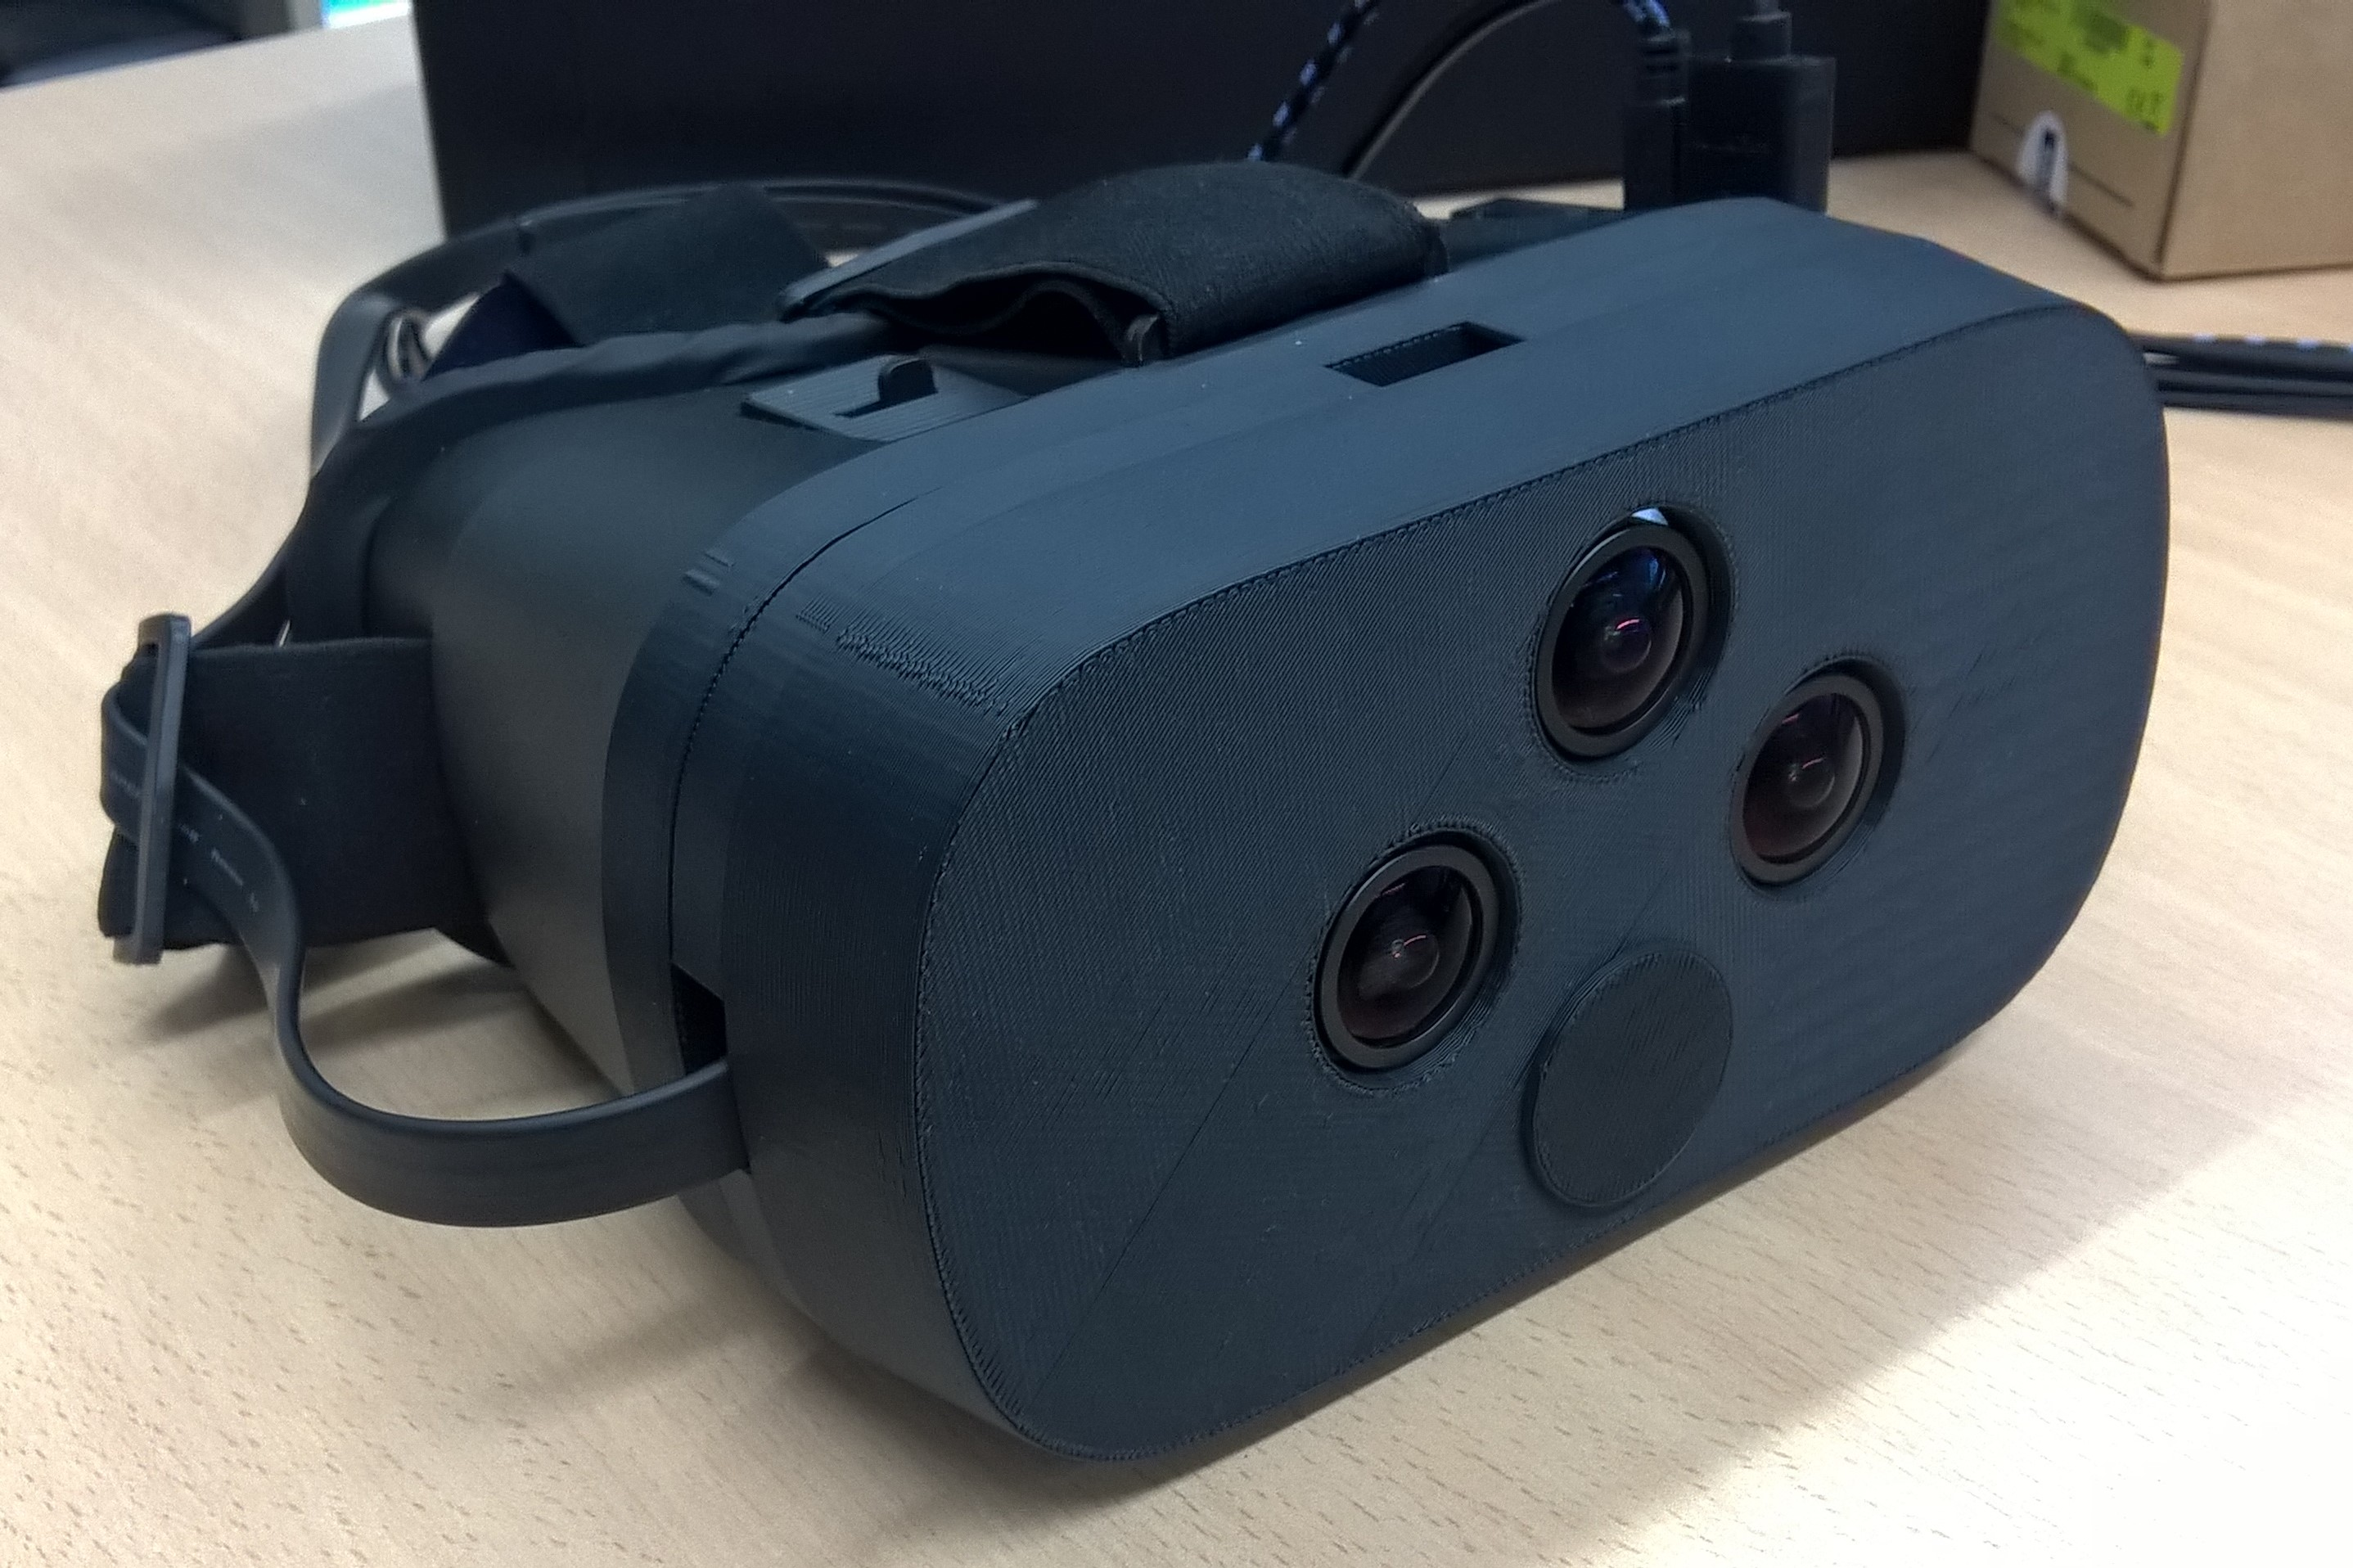
\includegraphics[width=1\linewidth]{img/imagenproto3.jpg}
		\caption{Current version of the HMD video-see-through prototype.}
		\label{fig:proto}
	\end{figure}
	
	As both types of devices are able to show different images for each eye, these systems are able to give the user stereo experiences, allowing the user to sense depth in the displayed images. 
	
	This project originated from the need to establish and resolve the reasons why the users have a poor experience, dizziness and eye strain, when using video-see-through devices. As is explained in \cite{disconfortReview} and was experimentally tested in \cite{vergenceDisconfort}, the Accommodation-Vergence conflict is one of the issues that causes this poor user experience.
	
	The vergence is the process where the eyes set their angle of visualization trying to fuse the image of an object keeping it into sharp focus, whereas the accommodation is the process where the objects difficult to fuse are blurred. Both process are tightly coupled giving each other feedback in order to keep the images as sharp and fused as possible. 
	
	The issue arises as a result of using near eye screens to show stereo 3D. In these displays the image is shown always at the same distance of the eye, however, the distance between objects, disparity,  changes when the environment is changed. For example, changing from looking at a distant object to a close object.  This conflict can be observed in Fig.\ref{fig:vergence}.
	
	\begin{figure}
		\centering
		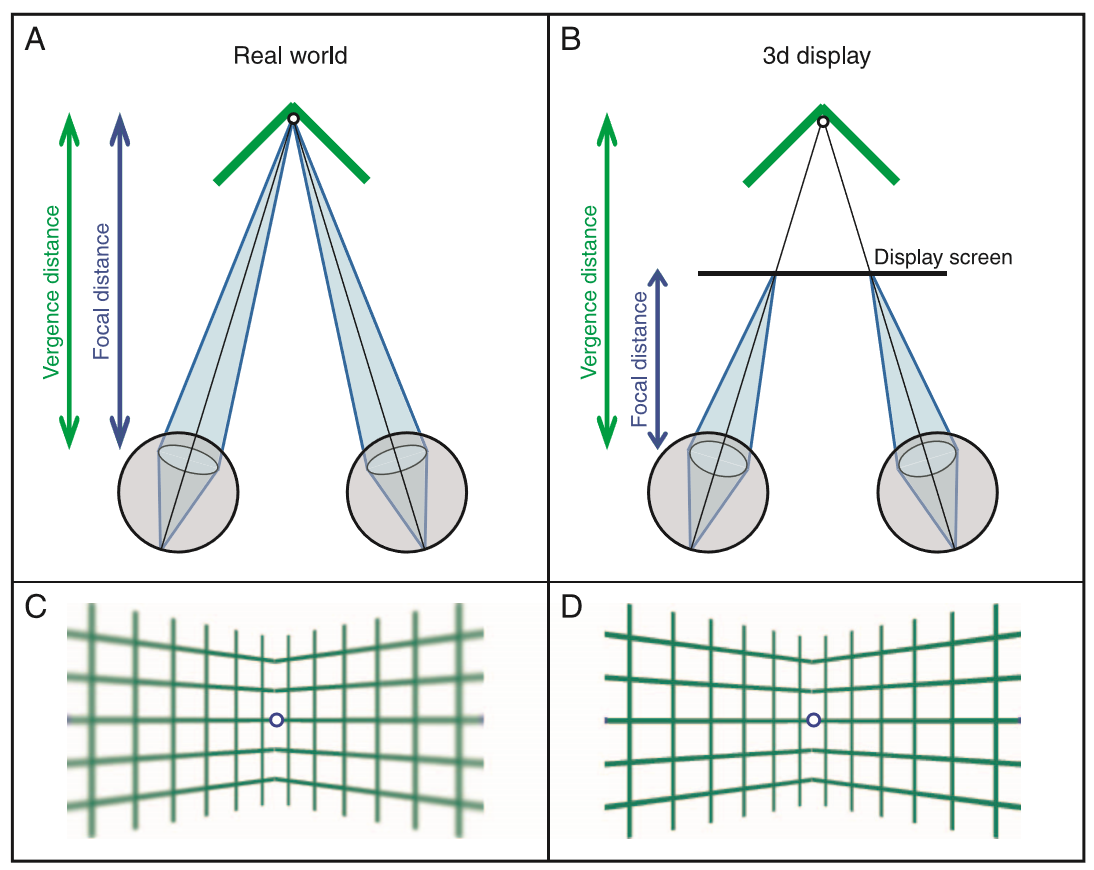
\includegraphics[width=1\linewidth]{img/vergencia.png}
		\caption{ In A and C can be seen the usual effect that happens when the coupling of the accommodation vergence is correct. As the accomodation distance is the same as the vergence distance, a blur effect appears in the corners. In B and D can be seen the effect that happens when an stereo scene is showed through near eye screens. As the accomodation distance is different than the vergence distance, no blur effect is applied in the corners. Source \cite{vergenceDisconfort}.}
		\label{fig:vergence}
	\end{figure}
	
	Parallel to the accommodation vergence conflict, another issue that occurs when using video-see-thought is that objects seem to have different sizes than in the real world. This is an important issue when the user is trying to grab or manipulate objects and generally when the user is estimating distances. This issue happens because the camera is not in the same position as the eyes producing an error in the size perception.
	
	Consequently, this project tries to solve the Accommodation-Vergence conflict and the size issue using environment information to set the distance between images of the viewer and change size settings.
	
		
	\section{State of the art}
	\label{sec:art}
	%explicar de donde viene el vr, hacia donde va, tecnicas tipicas usadas para resolucion del problema de la vergencia (seguimiento de los ojos), hablar de tecnicas de depth map
	%- hardware que se utiliza ahora, problema y incovenientes
	%- depth map, Libelas, explicar que existe la middlebury datebase y porque hemos elegido libelas???????????????????
	%- calibration (?) explicar en que consiste
	The Accomodation-Vergence conflict is a topic of great interest in the research field, therefore, a wide variety of  solutions have been proposed to try to solve this problem. 
	
	One of the many solutions found to ease this problem is applying blur to zones where the images not fuse correctly, this simulates the effect that the user would experience if the conflict would not have happened, see \cite{neareyeblur}. Related with this, a research \cite{sceneComposition} found that placing objects connecting different depth planes help the users to better transition between objects aiding to maintain the coupling between accommodation and vergence. Other line of research is to use eye-tracking techniques \cite{eyeTracking}. These technologies allow the system to know where the eye is looking on the image and then blur the out of focus areas. 
	
	After all of this, we can see that this project takes a different approach compared with the main lines of research.  This project uses depth data collected from a stereo camera placed in front of the headset to change the distance between images inside the headset. However, to get the depth information a reliable and fast stereo matcher was needed. That is why ELAS\footnote{Acronym from Efficient large-scale stereo matcher.} \cite{LIBELAS} and its implementation LIBELAS were used.
		
	In the stereo matcher field, two main branches can be found, local stereo matchers and global stereo matchers. Global stereo matchers are reliable but use many compute power. On the contrary, local stereo matchers are fast but less reliable than the global matchers. ELAS first uses a global stereo matcher on highly reliable points and after removing the more redundant, a Delaunay triangle mesh is created from that points. After that, the regions are then processed by a local stereo matcher. More information about ELAS implementation can be found on \cite{LIBELAS}. 
	
	Using LIBELAS though, introduces a new requirement. It requires that the input image pair must be rectified before it can be used. This is because libelas uses the epipolar lines\footnote{In stereo systems, a geometry relation between points from one image to the other. }, to find the disparities between images, this is done because is faster than searching over the hole image. For that reason, a calibration module to correct the image distortion, rotation and translation is needed. To solve this issue, OpenCV calibration functions were selected, their implementation is based on \cite{bouguetcalibration} and \cite{calibrationopencv2}. An example of this can be found on the appendix \ref{fig:rec}.

	\section{Objectives}
	After the previous analysis and explanation of the problem, the main objectives of this project are the following: 

	\begin{itemize}
		\item Evaluate the user experience when using the HMD and determine whether the accommodation-vergence effect causes dizziness and general discomfort on the users. 
		
		\item Evaluate on one hand if the user perceives incorrectly the distances and sizes of the objects when using a video-see-through HMD. And in the other hand whether this issue supposes a problem for the users.
		
		\item If the Accomodation-Vergence is one of the causes of the discomfort on the users, the problem will be solved using the deph information that can be obtained using stereo vision. 
		
		\item If the user perception of size and distance when using a HMD is an issue, solve it by adapting the visualization of the scene to the distance of the objects within it.
		
		\item Evaluate the user experience after the development and conclude whether our approach for solving these problems reduces the discomfort of the users. 
		
		\item Add the required modules keeping in mind the usefulness of these for future developments.
		
		\item Integrate all the required modules in the visualization program without reducing the performance. 
	\end{itemize}

	\section{Methodology}
	%dudas sobre este apartado
	%hablar de tecnicas de desarrollo agil y sobretodo de las librerias utilizadas y de las limitaciones y ventajas que estas nos han aportado.
	
	%Scrum and its variants are one of the most spread work methodologies nowadays. Therefore we believe convenient to use it as one of the foundation of this project, however, as this project was only done by one person, some changes were made. 
	
	The Scrum methodology was selected as one of the foundations of this project. However, as this project was only done by one person, some changes were made. 
	
	As there was only one developer, the daily meeting was replaced with a weekly meeting with the project supervisors, in this case the tutor and the boss of the laboratory department in the CVC. In these meetings we evaluated the development done, the issues faced that week and the problems solved. Related with the Scrum methodology, Github \cite{web:github},\cite{web:githubDesktop} was used as version control system and Trello\cite{web:trello} as the task manager system.
	
	Involving the tools used to develop this project, C++ and QT \cite{web:qt} were used mainly because the previous development of the visualization system was done using that environment. QT libraries were used to develop the interface and the visualization of the images on the screen. In addition, OpenCV was used as the library for image processing and calibration, \cite{web:opencv}. Some code snippets for testing and evaluation of the results were done using Matlab\cite{web:matlab}. 
	
	
	\section{Tools and Development}
	
	First the tools and modules developed will be presented and after the pipeline and integration of the parts will be explained. 
	
	\subsection{Calibration}
	\label{sec:calib}
	%en este apartado hablare sobre que tecnicas se han usado para realizar la calibracion y como se ha implementado y %estructurado, explicar problemas encontrados para la calibracion (descalibracion constante parametros utilizados)
	
	The calibration module is a key item inside the pipeline to be able to get the LIBELAS depth map. This module can be split in several parts:  
	
	First, a dataset of captures of a chessboard pattern have to be taken to get references of the distortion, rotation and distance of the cameras. In these images the pattern has to be visible by both cameras and cannot be occluded neither be partially out of the image. In addition, the dataset must contain images of the pattern in various positions, the more locations covered by the images the better the results of the calibration will be. 
	
	Second, once the dataset is obtained, the next step is locating the chessboard pattern inside each image, to locate these points an OpenCV function is used first to find them and after to make these points more precise. In this step each camera dataset will be processed independently. 
	
	Once the points are calculated, they are passed to the monocular calibration function of OpenCV to obtain the intrinsic matrix and the distortion vector.  Although these parameters per se can be used in a undistortion function to remove the image distortion, we need a stereo rectification because monocular calibration does not take into account the traslation and the rotation between cameras. For that reason, a stereo calibration is needed. 
	
	After the monocular calibration, these matrices along with the image points are passed to the stereo calibration function and the resulting matrices passed again to the rectification function. Once this function is finished we now have the projection and rotation matrices from both cameras. These can be passed to the undistortion function along with two images to rectify the distortion and align both images in the same epipolar lines. Alternatively, these matrices can be passed to a undistort mapping function for faster undistortion of the images.  
	
	Some problems were faced during the development of this module. The main issue was that some adjustment had to be done in the configuration parameters of the OpenCV function because excessive undistortion was done over the images leaving them completely unusable. The parameters adjusted were the number of coefficients from the distortion vector used by the calibration modules. 
	
	All of these matrices and configurations can be saved and loaded to avoid the need to calibrate each time the program is started.  
	
	\subsection{Libelas}
	\label{sec:libelas}
	 This module starts with two images that have already been undistorted with the stereo calibration, these then are passed to the LIBELAS processing function, this function computes the disparity from two given images and returns two disparity maps, one for each given image. These maps indicate us the distance between one pixel from one image to the other.  
	 
	 One of the problems faced by this library, and in general by depth map stereo matchers, is the existence of low textured areas on the image, this can be observed in \ref{fig:disparity} on the white area of the opthalmologic pattern. These regions usually end up without disparity values, therefore, potentially producing issues in further processing. These regions along with occluded ones and calibration faulty areas are usually set to negative values by Libelas itself, therefore can be easily detected.  
	 
	 These maps can be visualized in grayscale by changing the range of the image or with a colormap to better appreciate the depth gradient. 
	 
	 One issue faced during the development of this module was the extremely high calibration precision needed in order to get quality images. The cameras, not totally fixed in position, usually moved slightly, reducing the quality of the depth map obtained. The issue was communicated to the hardware development team in order to change the HDM prototype to better secure the cameras position.  
	 
	 Although LIBELAS is a fast library it was not quick enough to process the images in real time or near real time, to solve this issue, two possible solutions were found. 
	 
	 \begin{itemize}
	 	\item The first idea was to apply a ROI in the center of the images after the distortion, that way as the image is smaller, requiring less computing power to be processed. As the image is only cropped, it will keep all the details of the center of the image, where the user will be usually looking at.  
	 	 
	 	\item Other idea was to make down sampling of the images before using them on LIBELAS. This also decreases the computing power required to process the images, however it also decreases the detail of the image, potentially affecting the quality of the depth map.  
 	 \end{itemize}
	 %In \ref{sec:roiresize} a comparison between both methods can be seen. 
	 
	 To improve the quality of the depth map obtained in LIBELAS the default configuration called "Robotics" was taken as base and modified. First, we added the configuration that enables support points to be in the corners. We also removed the postprocessing features like median filtering or mean filtering. These last changes improve the speed and fit better with the environment where the testing was developed.
	 
 	\begin{figure}
 		\centering
 		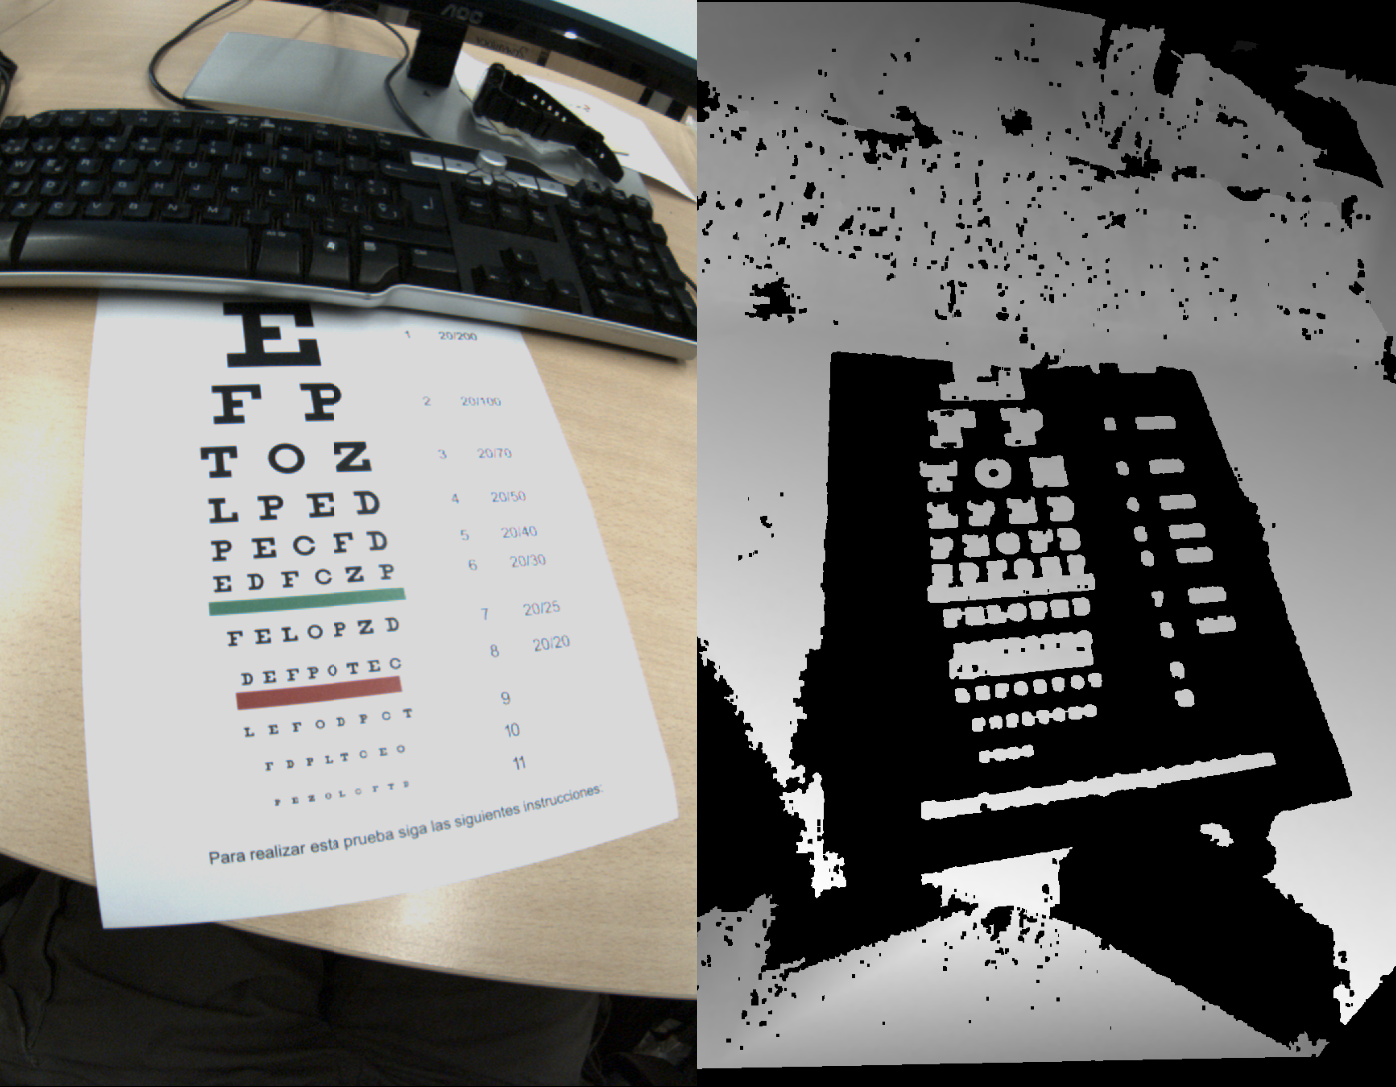
\includegraphics[width=\linewidth]{img/depthdistort.png}
 		\caption{At the left the original image, and at the right the depth map. Can be noticed the lack of disparity values in the area of the pattern.}
 		\label{fig:disparity}
 \end{figure}
	 
	 
	 
	\subsection{Configuration}
	
	Users have different vision systems between them, for example different eye sizes, different distance between eyes, etc. All of this must be taken into account as it influences the user experience. Also users should be able to adjust each configuration to the distance of the viewed objects.  For these reasons the following modules were developed.
	
	First, a module able to modify the position of the images over the screens of the HMD was implemented. This module is designed to show only a ROI of the full resolution output of the camera, letting the user decide and change every possible aspect of this ROI, from the size of the ROI to the anchor point. These parameters can also be saved to be used in other sessions or to be able to change between different settings for different distances. Once the ROI is obtained graphic functions from QT are called to display them on the screen.
	
	Second, a module capable of make transitions between settings was developed. This module calculates the distance between two settings and does the transition in a given number of steps. It transitions the movement in two phases, first adjusting the zooming and then changing the position of ROI.
	
	\subsection{Pipeline and module integration}
	\label{sec:pipeline}
	
	Parallel to the development of said modules, a pipeline integrating them was built. This pipeline has the goal of combining the developed module to achieve a real time dynamic system that changes between already set configurations to adapt to the scene variations. This pipeline had to be fast and have quick response times, for that reason it was decided to use a threaded architecture to allow each thread to perform their tasks at their own pace without harming the performance of the thread in charge of updating the screen. This helps to reduce the reaction time improving the user experience. 
	
	A simple classifier has been developed to determine which distance the user is currently viewing. It uses the output of LIBELAS to perform a operation (mean, max or min) over the disparity map. The output value is then used in a threshold classifier to select between 3 different distances, near, medium and far. 
	To assure stability on the output of the classifier the output of the last frames are saved and then a mean is calculated between the current value and the previous ones. The ouput of this  is used as the input for the threshold classification. 
	
	As can be seen in Fig.\ref{fig:pipeline} the pipeline can be split in the following parts: 
	
	\begin{itemize}
		\item Grabbing threads: these threads grab images from the cameras that are set to be continuously capturing frames. After that, the images are then stored on a variable overwriting the previous image. This thread is continuously looping to grab the most recent image.
		
		\item Processing threads: this threat uses a image pair placed by the displaying thread to classify the image distance. This images will be undistorted first and then passed to LIBELAS to obtain the depth map. After that the central region is cropped and the image is passed to the classifier. Finally, the output classified distance is stored on a variable which will be queried each iteration by the displaying thread.  
		
		\item Displaying thread: the goal of this thread is to obtain the images from the grabbing threads and display them on the screen of the HMD. For this it uses the ROI module to set selected configuration. After the ROI is done, the image is mapped on the QT graphic scene. QT then rescales the image to fit it on the screen of the device. This is used as a zoom since if a smaller region of the image is cropped it will be rescaled and the objects would look bigger. This thread also passes the images grabbed to the image processing thread, and uses its output, the classified distance, to dynamically select between user settings. Also, if set, it will use the transition module to smooth the change between settings. 
		
	\end{itemize}
	
	\begin{figure}
		\centering
		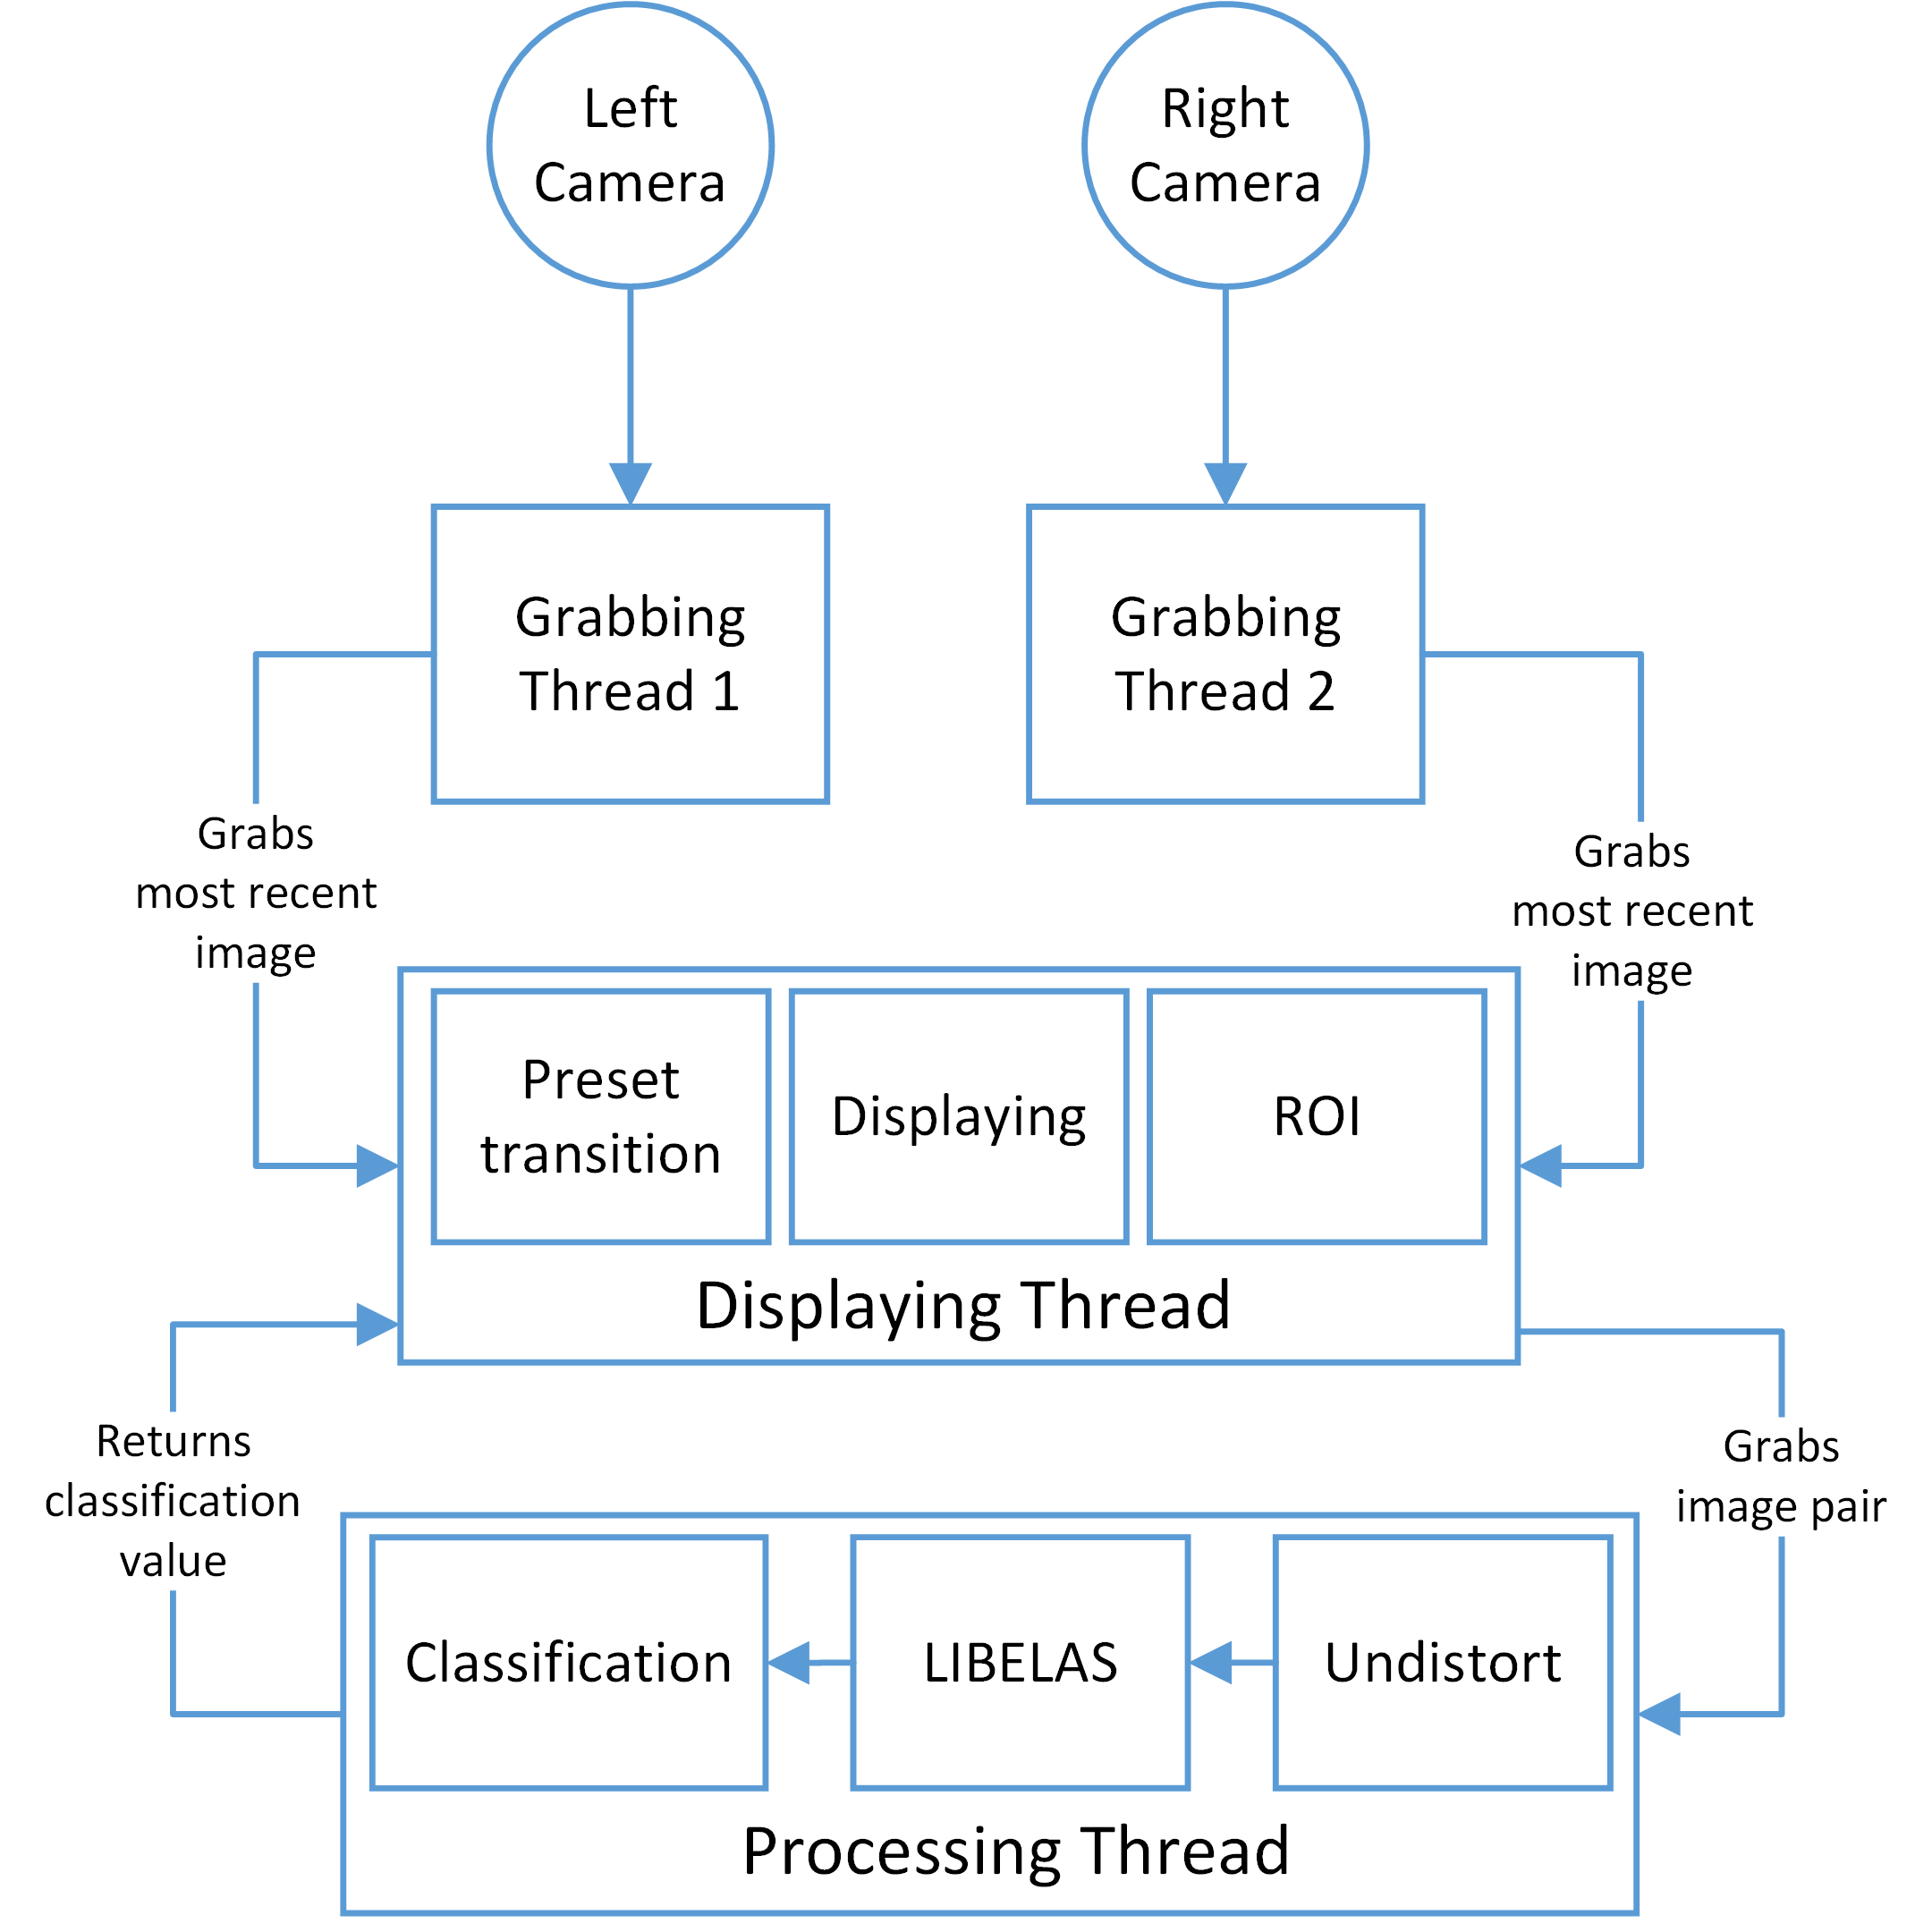
\includegraphics[width=1\linewidth]{img/pipeline.png}
		\caption{Diagram of the pipeline of the system. At top the grabbing threads that capture the images from the cameras. In the middle the thread that displays the images and changes between user settings. At the bottom the thread that process the images and classifies them. }
		\label{fig:pipeline}
	\end{figure}
	
	
	\subsection{Offline pipeline}
	One of the issues, was that LIBELAS was not able to produce real time processing. For that reason, a video recording and processing modules were also implemented.  
	
	The module was developed using OpenCV functions for video reading and recording. This videos were intended to be saved in raw format, but due to an unresolved bug in the OpenCV modules that prevented the reading of raw videos, the videos were saved instead using the Intel's IYUV codec. %As it is lossless, the images are effectively the same as the images on the online pipeline.
	Other problem related with the recording module was that the videos have to be saved in memory, because storing them directly on disc is not possible. That is because of the slow writing speeds of the hard drive that will not be able to keep up with frame generation of the cameras, therefore not storing all the captured frames. Despite that, another issue was faced because the size of the in-memory stored images would rapidly increase overpassing the size limit imposed to 32 bits software. For this reason the whole project was modified to be compatible with 64 bits architectures.
	
	After the implementation of this module an offline pipeline was developed to allow the processing of these videos. The architecture is similar to the online pipeline seen in \ref{sec:pipeline}, but has some noteworthy differences.  
	
	First, as it is not necessary this pipeline does not use a threaded architecture.
	
	Second, the images are read from a video instead of a camera, as the frames from the video can be grabbed on demand, every frame can be processed. The input video can be already undistorted or if that is not the case, the images are undistorted using the calibration module explained in \ref{sec:calib}. 
	
	Third, after the frame is processed by LIBELAS, the output depth map can be converted to a grayscale or colormap image and be saved in another video for further processing or viewing. Alternatively the images can be evaluated in place using the threshold classifier already explained.  
	
	%explicar analisis de los resultados usando matlab

	
	\section{Results}
	
	%\subsection{Calibration Comparison}
	%comparaciones entre imagenes no calibradas y imagenes calibradas
	%en este apartado compararemos las imagenes originales con calibracion obtenida via opencv y la obtenida via %matlab (quizas es un poco innceseraio este apartado ?)
	
	\subsection{LIBELAS performance}
	\label{sec:resizeperformance}
	In \ref{sec:libelas}, we explained that the processing module was not fast enough when using full-sized images due to LIBELAS high computing time. To solve that, two solutions were developed. Cropping the center of the image and reducing the size of the images using down sampling. In Table \ref{tab:timeprocess} can be seen that, as expected, a ROI with half the resolution is 4 times faster. Also, as down sampling is more compute intensive it is slightly slower than using the ROI.  
	
	Is also remarkable that as the image resolution is reduced, LIBELAS stops being the main bottleneck of the processing module going from 90 \% of the computing time to 50 \% when the image is 4 times smaller and to a 10 \% when the image is 12 times smaller, see Fig.\ref{fig:libelaspercentatge}. This bottleneck has been transfered to other time consuming tasks like the rectification.
	
	With these results, we can conclude that the time difference between cropping the images and resizing is minimal and that from one point is irrelevant further reduction of the image as the framerate will not benefit from it.  
	
	\begin{table}
		\centering
		\begin{tabular}{@{}cccc@{}}
			\toprule
			Time (ms) & Original & ROI & Down sampling \\ \midrule
			LIBELAS   & 581      & 128 & 135           \\
			Rectify   & 16.9     & 16  & 16.1          \\
			Total     & 624      & 156 & 165           \\ \bottomrule
		\end{tabular}
		\caption{Computing time of LIBELAS, the rectification and all the processing module in milliseconds in 175 frames from a near distance video.}
		\label{tab:timeprocess}
	\end{table}
	
	\begin{figure}
		\centering
		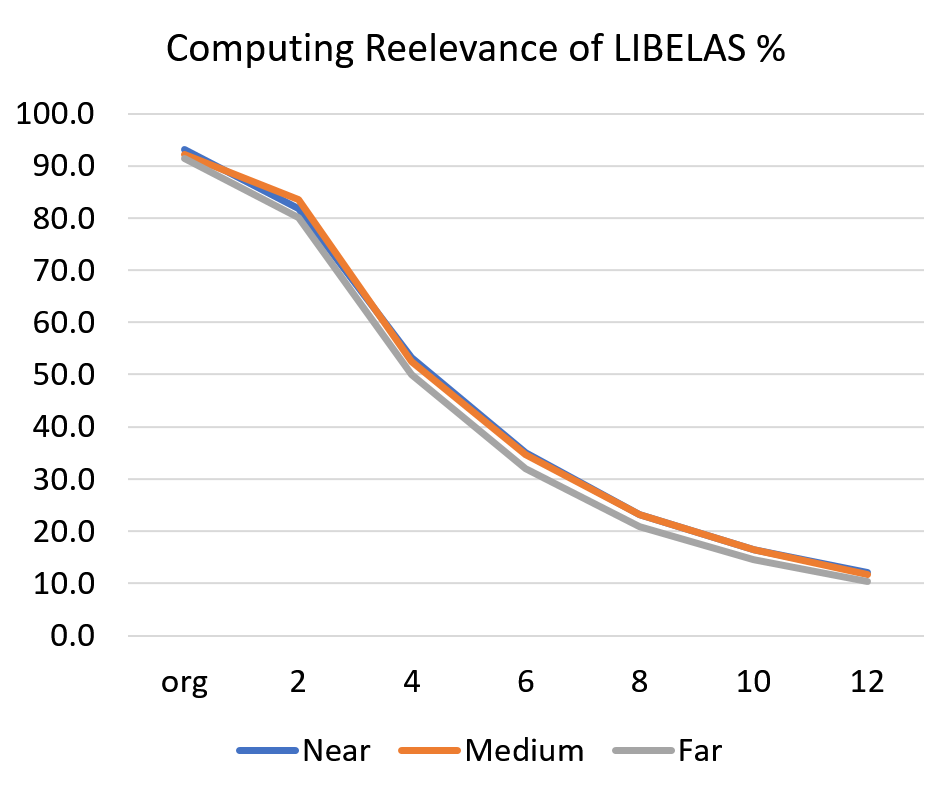
\includegraphics[width=1\linewidth]{img/ComputingLibelas.PNG}
		\caption{Computing time of LIBELAS in percentage over the total processing time in 3 different videos with different distances.}
		\label{fig:libelaspercentatge}
	\end{figure}
	
	\subsection{LIBELAS output}
	\label{sec:libelasOutput}
	As explained in \ref{sec:pipeline}, before applying the classification, the output of LIBELAS is cropped and an operation is performed, mean, maximum or minimum. This value is then used as input for the threshold classifier.  
	
	It is important that the input values for the classifier are stable to keep the settings changes as minimum as necessary. This is because these changes disturb the user perception and if this happen repeatedly in a short amount of time, they could induce motion sickness to the users.  
	
	On the one hand in Fig.\ref{fig:output:mean} can be observed that the output value of the mean operation is stable, being the only one with a clear separation of the values in all the tested sizes. From these results can also be deduced that there is no need to use the full-sized resolution on the images as it is slower to process, see \ref{sec:resizeperformance}, and it does not yield better results for the classification. 
	
	On the other hand, the output of the minimum and the maximum operations, Fig.\ref{fig:output:min} and Fig.\ref{fig:output:max}, cannot be distinguished correctly. When the minimum operation is used the medium and the far distances cannot be split in different classes because their values overlap between them. A similar case happens also with the maximum operation, in this case though it only happens to the original size. %, this can be due to 
	
	Looking at the ROI chart, can be seen that with a ROI 4 times and 12 times smaller than the original size, yield atypical results. This can be notice in the 4 times roi, where the near distance obtains less disparity than the medium one and in the 12 times ROI where the disparity is totally inversed. This is not possible because disparity, is linked with the distance between objects, closer objects have bigger disparities. What is happening is that LIBELAS is not capable of extracting the depth information from these images because it is not able to find reliable support points, therefore, returning inaccurate depth maps. 

	\begin{figure}
		\centering
		\begin{subfigure}[t]{0.5\textwidth}
			\centering
			\includegraphics[width=\linewidth]{img/mean2.png}
			\caption{Mean operation with down sampling.\newline}
			\label{fig:output:mean}
		\end{subfigure}
	
		\begin{subfigure}[t]{0.5\textwidth}
			\centering
			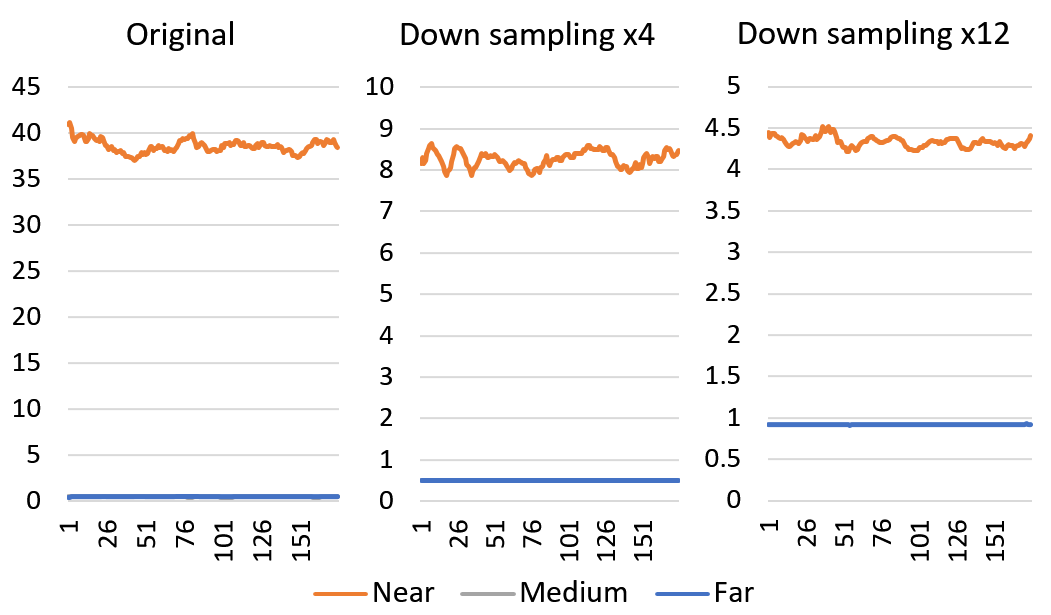
\includegraphics[width=\linewidth]{img/min2.png}
			\caption{Minimum operation with down sampling.\newline}
			\label{fig:output:min}
		\end{subfigure}

		\begin{subfigure}[t]{0.5\textwidth}
			\centering
			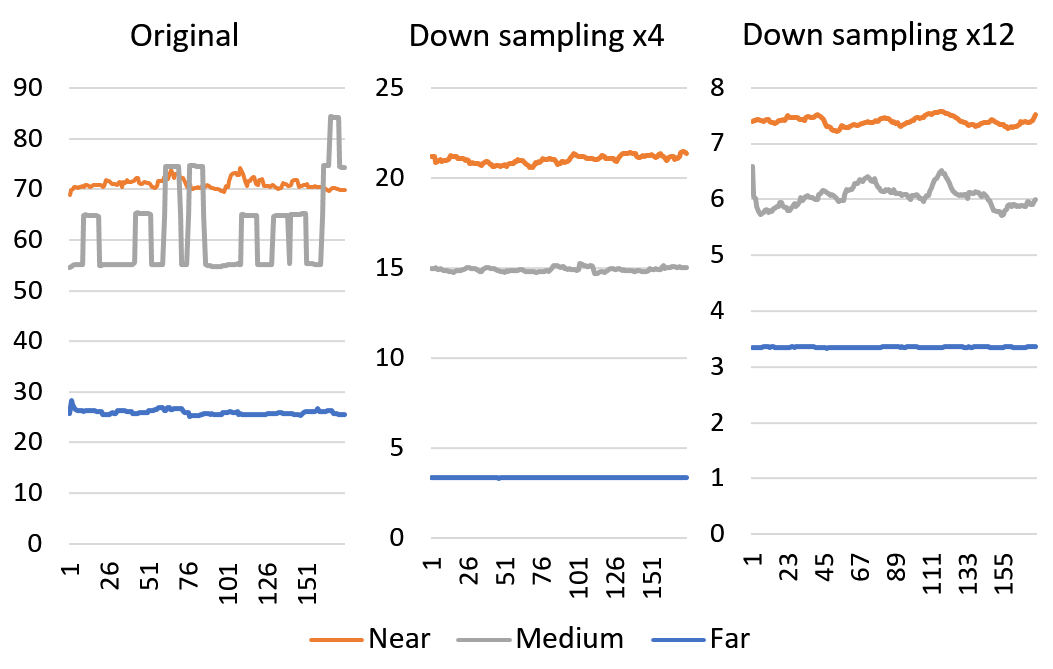
\includegraphics[width=\linewidth]{img/max2.png}
			\caption{Maximum operation with down sampling.\newline}
			\label{fig:output:max}
		\end{subfigure}

		\begin{subfigure}[t]{0.5\textwidth}
			\centering
			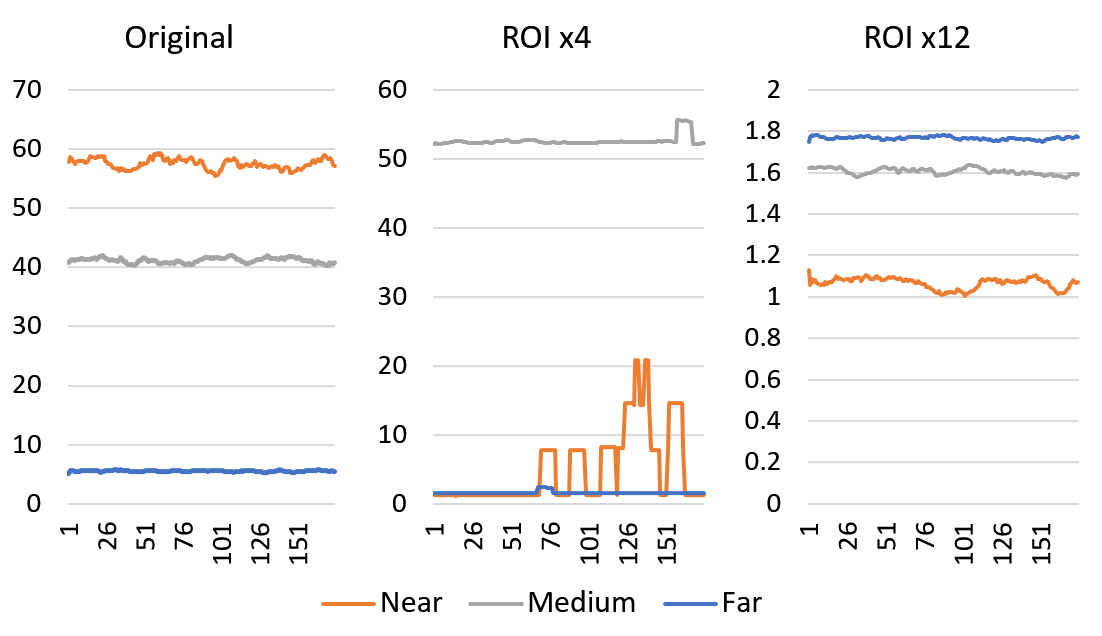
\includegraphics[width=\linewidth]{img/roimean2.png}
			\caption{Mean operation with ROI cropping.\newline}
			\label{fig:output:roicrop}
		\end{subfigure}
		\caption{ Charts of the output of the operation over the center of the depth map with different operations on different sizes and distances.}
		\label{fig:output}
	\end{figure}
	
	\subsection{First user testing}
	
	In the first user testing session, the goal was to carry out a preliminary evaluation on the Accommodation-Vergence conflict and in the issue of the size of the objects. The protocol followed in this user testing session can be found in the appendix \ref{sec:annex:user1}.
	
	The results of this first user testing session can be seen in Table \ref{tab:firstUserTestResults}. One main thing can be noticed, two of the six users that participated in the user testing sessions did only change slightly the parameters of the configuration. 
	While the other users did changed the configuration. This is important because the users that did not change much the distance between image said they did not felt dizzy when using a setting in different distance than the original. On the contrary, the users that did change the distance between images mostly felt dizzy when using a setting set for a different distance than they were seeing.
	
	At the same time, it was noticed that in most cases, both types of users felt that the objects were further away when using the close setting in large distances, and vice versa in case of far settings in closer distances. This confirms that a solution is needed to reduce this issue. 
	
	After this user testing session, it was agreed that a new user testing session have to take place to evaluate and resolve some of the problems faced in this one. 

	First we need to ensure that the users like S1 and S3 are correctly seeing the stereoscopic 3D and if this results repeat in different testing conditions. It is possible that the default setting was similar to their comfortable setting and therefore they did not think relevant to change it. For that reason in further user testing sessions a the default setting will be set to have a huge displacement on the X axis, forcing the users to always move their setting to the better fitting for them.
	
	Second, some users found difficult to set the vergence in the closer distances for lack of a relevant 3D object or form, for this reason in further user testing an object could be introduced into the test to ease the setting up. 
	
	Third, during the testing of the settings in other distances, testing in the distance where the setting was set up may be necessary to ensure that the user have set correctly that distance.
	
	Fourth, we noticed that some users found it difficult to find the keys used to move the images, for that reason we decided to move the keys that change the position of the right image from i,j,k and l to the arrow keys. 
	
	Fifth, after the testing was done we noticed that the cameras were slightly out of focus and the brightness, contrast and color balance was not correct, as this can also impact on the user comfortability, from now on before every user testing session, the general camera configuration will be checked.
	
	
	\begin{table*}
		\begin{center}
			\begin{tabular}{cccccccc}
				\toprule
				& & \multicolumn{2}{c}{Near} & \multicolumn{2}{c}{Medium} & \multicolumn{2}{c}{Far} \\ 
				Subject &Feelings & $\Delta X$ & $\Delta Y$ & $\Delta X$ & $\Delta Y$ & $\Delta X$ & $\Delta X$ \\ 
				\midrule
				S1&Confortable & 0 & 6 & 3 & 0 & -9 & 0 \\ 
				\midrule 
				S2&Disconfort & 3 & 0 & -129 & 0 & -57 & 30 \\ 
				\midrule
				S3&Confortable & 3 & 0 & 3 & 0 & 3 & 0 \\ 
				\midrule 
				S4&Disconfort & 3 & -3 & -33 & 12 & -36 & -3 \\ 
				\midrule
				S5&Disconfort & -12 & 0 & -66 & 0 & -42 & 0 \\ 
				\midrule
				S6&Disconfort & -24 & 0 & -39 & 5 & -45 & -6 \\ 
				\bottomrule
			\end{tabular} 
			\caption{Results of the configuration of the ROIs in the first user testing session. The second column represents the general feelings of the users when changing the settings. Note that $\Delta X$ means separation between the center of the image pair in the X axis and $\Delta Y$ means separation between centers in the Y axis.}
			\label{tab:firstUserTestResults}
		\end{center}
	\end{table*}
	
	
	\subsection{Second user testing}
	%en este apartado mostraremos los distintos resultados obtenidos en la segunda sesion de user testing , explicaremos los resultados y concluiremos si nuestra hipotesis es correcta y si la solucion desarrollada es suficiente para resolver este problema, en caso de que no, nos plantearemos cuales son o han sido los problemas que impiden que el usuario sienta una mejora al utilizar la vergencia dinamica.
	
	For this second user testing session the goal was to evaluate whether the Accommodation-Vergence conflict and the issue of the size of the objects affect all the users and whether the dynamic setting changer solves this problem. After the evaluation of the latest user testing some considerations were concluded. These have been taken into account in this second user testing with the goal of improving the consistency of the results. 
	
	Following the considerations of the last user testing, the right image was totally shifted with a starting difference between center points in the x axis ($\Delta X$\footnote{For simplicity  $\Delta X$ and $\Delta Y$ would be used as an abbreviation for the difference between the position of the centers of the ROIs on the X and Y axis. }) of +158 pixels. This should force the users to adjust the setting and not be comfortable with the default configuration. Also a small cardboard box was used instead of the opthalmologic pattern to aid the configuration of the near settings. More detail of the protocol can be found in the annex \ref{sec:annex:user2}.
	
	Note that in this user testing subjects S1 and S3 from the first user testing session also participated in this session. This would allow us to evaluate if they still feel comfortable without changing the parameters or if all was a misunderstanding and they also need to change the configuration to feel comfortable. 
	
	\subsubsection{Accomodation-Vergence settings}
	The first thing that can be noticed from Fig.\ref{fig:ut:2:deltax} is that every user more or less changed the gap between images to feel more comfortable with the distance currently viewed. Even the subjects S1 and S3 did change the gap. From these results can be deduced that the larger the distance is, the greater the separation between the images will be, since negative values mean greater distance between images. 
	
	It is possible though that with more further away objects, the increase of the distance between images will reduce, arriving to cap where more separation is no further needed. This is because the disparity between the images received by the eyes decreases when the objects are moved further away.
	
	Also is noticeable that the variation on the $\Delta X$ is bigger on the closer settings, this can be caused by the fact that slightly movements or variations are more significant when the distance between the user and the object is lower. 
	Finally, as was expected this difference is not seen in the Y, this is because the Accomodation-Vergence issue is related with the disparity in the X axis. 
	
	\begin{figure}
		\centering
		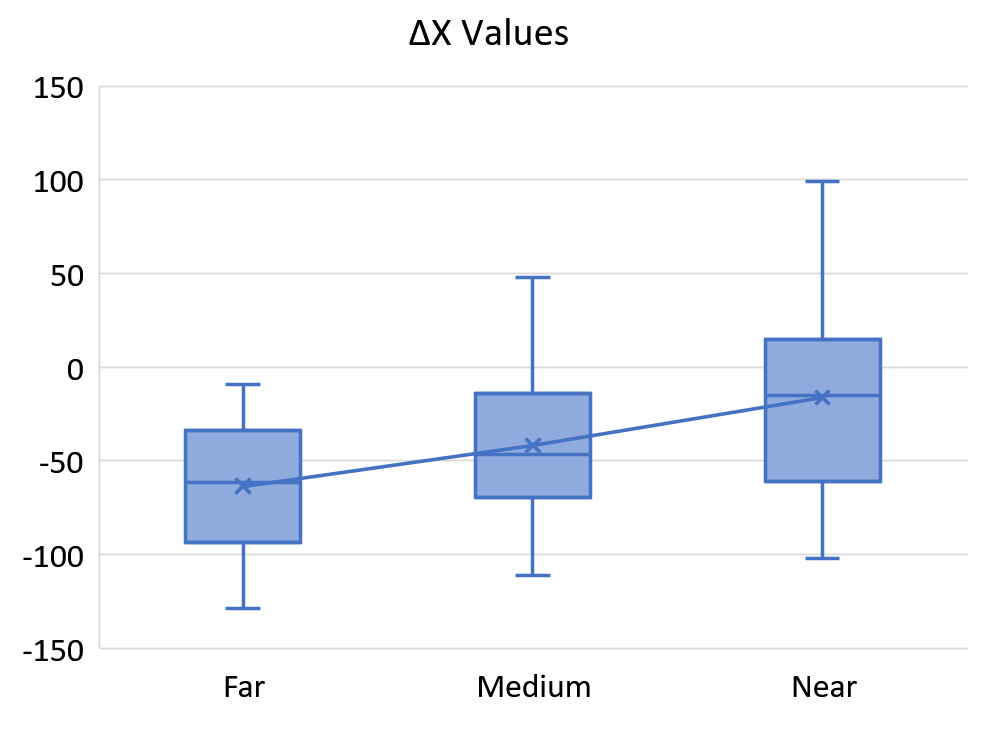
\includegraphics[width=1\linewidth]{img/fancydelta.png}
		\caption{Mean distance between center points of the images on each configuration. Note that $\Delta X$ means separation between the center of the image pair in the X axis.}
		\label{fig:ut:2:deltax}
	\end{figure}
	
	\subsubsection{User opinion of the settings }
	Looking now at the user experience when using a setting in a different distance, see Fig.\ref{fig:ut:2:deltax} and Table \ref{tab:ut:2:feelings}. Can be noticed that users feel more comfortable using a setting at the original distance which it was set in. One noticed also that only 58.3\% of the users felt comfortable with the distance when using the distant setting in a distant environment. This also happens with the medium setting. On the contrary 83\% of the users said that they felt comfortable when using near configuration in near environments. This difference can be related with the fact that users in the near set up can interact with the objects therefore better fitting that configuration. 
	
	As the medium setting has the more intermediate values, is almost usable on every distance, thought this does not mean that would be comfortable to use it. More than half the users do not feel comfortable when using this medium setting on far distances. As expected, far and near configurations perform worse when used in the other's distance.
	
	After these results can be concluded that a module capable of changing the setting will be convenient to improve the user experience. 
	

	
	\subsubsection{Size issue}
	
	In Fig.\ref{fig:ut:2:size} a comparison is shown between the mean size of the ROI in every configuration. With these results it is clear that each distance needs a different size setting.  The users set smaller ROIs, bigger zooms over the image, to distant objects, seeing that objects bigger. On the contrary the users set bigger ROIs, smaller zooms, to closer objects, seeing them smaller. This results follow the expected pattern. A system capable of automatically changing the between settings would solve this problem. 
	
	\begin{figure}
		\centering
		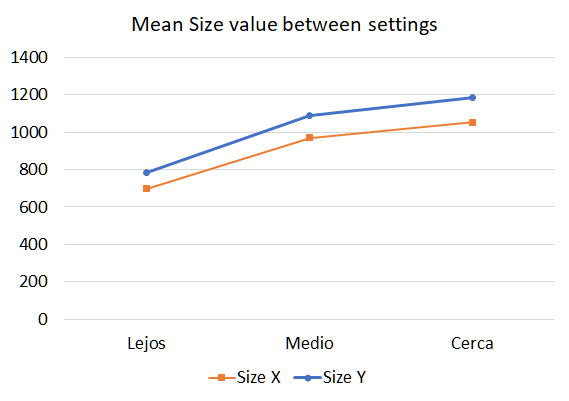
\includegraphics[width=1\linewidth]{img/userTestingSizechart.png}
		\caption{Mean size of the images in each configuration for each distance. Note that a bigger size means a bigger ROI and therefore smaller objects.}
		\label{fig:ut:2:size}
	\end{figure}
	
	\subsubsection{User opinion on the dynamic settings}
	As the pipeline was already finished, this user testing session also included a test of the system with the full pipeline working, capable of changing between configurations. This module was used after the user had already set every configuration for each distance.  
	For the user testing, the mean of the central region of the 10 last images were saved to preserve stability in the output of the classification. None of the users complained about undesired changes of the settings when using this system.  
	
	First of all, all the users agreed that changing the parameters dynamically is better than having one setting for every distance and it is more convenient than having to change the setting manually. Also all agreed that after changing from one setting to the other no adaptation period is needed or it is short and not annoying.  
	
	In Table \ref{tab:ut:2:dynamic}, can be seen that a tight majority of the users prefer not having a transition period when changing dynamically from one setting to the other. This can be related with the users also saying that this transition was slow and that having two differentiable phases of transition was not comfortable. In the other hand some users said that not using transitions was too abrupt even though it does not induced dizziness. 
	
	It can be concluded that the usage of the dynamic setting changer improves the user experience by giving the user the most suitable configuration for each distance. But it is also clear that in the transition module there is margin for improvement as most of the users agreed that it was slow and not comfortable to see.
	
	\begin{table*}
		\centering
		\begin{tabular}{@{}cccccccc@{}}
			\toprule
			\multicolumn{2}{l}{\multirow{2}{*}{\% positive feelings}} & \multicolumn{2}{c}{Near distance} & \multicolumn{2}{c}{Medium distance} & \multicolumn{2}{c}{Far distance} \\
			\multicolumn{2}{l}{} & Fused & Size & Fused & Size & Fused & Size \\ \midrule
			\multirow{3}{*}{Setting} & Near & 91.7 & 83.3 & 33.3 & 50.0 & 0.0 & 8.3 \\
			& Medium & 91.7 & 50.0 & 83.3 & 58.3 & 45.5 & 33.3 \\
			& Far & 66.7 & 0.0 & 58.3 & 33.3 & 91.7 & 58.3 \\ \bottomrule
		\end{tabular}
		\caption{Results in the second user testing session of the feelings of the users in percentage of positive responses. At top the distance where the testing was done and at the left the configuration used when that response was given. Fused means if the user are seeing the images correctly fused, and Size if the users are seeing the object's size similar to the reality.}
		\label{tab:ut:2:feelings}
	\end{table*}

	\begin{table}
		\centering
		\begin{tabular}{@{}ccc@{}}
			\toprule
			& Dynamic & \begin{tabular}[c]{@{}c@{}}Dynamic +\\ Transition\end{tabular} \\ \midrule
			Preferences in \% & 58.3    & 41.7                                                           \\ \bottomrule
		\end{tabular}
		\caption{Preferences of the user when using the dynamic setting changer.}
		\label{tab:ut:2:dynamic}
	\end{table}




	
	\section{Conclusions}
	After the tests and the subsequent analysis were done, it was concluded that users experience dizziness when using HMD, this is related first, with the Accomodation-Vergence conflict and second by the issue with the size of the objects.
	Users have shown preference over the distance configuration that corresponded in each case to the distance they were seeing. This fits with the difference seen on the parameters of the configuration, where the users set the distance between images bigger when seeing distant objects and lower when looking at closer objects. 
	
	Also, was noticed that users set the zooming level depending on the distance they are seeing. For closer environments, the image is zoom out, meaning that objects are seen with smaller sizes. The contrary happens on objects seen in larger distances. User opinions during the testing also pointed that a different setting was needed to better fit each distance. All of this reinforced the idea that a system capable of changing between settings was necessary. 
	
	Despite some issues with the calibration and the performance of the depth map generation, the dynamic changer was successfully developed using the LIBELAS library. And the goal of improving the user experience was achieved as users that participated in the user testing sessions agreed that the experience was better when using the dynamic setting changer. 
	
	Related with the general performance, as the modules were build using a threaded architecture, the high computing tasks like generating the depth map or rectifying the images did not compromise the experience of the visualization. 
	
	
	\section{Future work}
	This projct is can be used as the foundation for many further research in the video-see-through HMD topic: 
	
	\begin{itemize}
		\item The depth map of this project can be used to generate augmented reality objects over the real-world.
		
		\item As was seen in section \ref{sec:art}, many researchers apply blur on the out of focus area of the image, to ease the Accomodation-Vergence conflict. Using the developed tools, we could go one step further using the depth map to apply this blur in objects on out of focus planes or applying it with more or less intensity depending on the depth. 
		
		\item This project can also be used to include more information on the environment by including a third camera with a different spectrum range.  
		
		\item Optimization of the software can be done to allow to use it on smaller and less powerful devices. 
		
		\item Related with the depth map, it would be interesting to compare between the latest depth map generators and see their time performance. 
		
		\item The transition module did not give as good feedback as was expected, users said that it was slow and uncomfortable to see. Therefore an improvement on this matter can be done and further user testing can be done to verify if a transition is needed or if is better to change the setting without any.
	\end{itemize}

	It is certain that this project has had some constrains that can be used as starting point for some research. These are mainly centered on the performance side. Improving the framerate and the image quality of the cameras is a thing that will happen over the years and will directly benefit the video-see-through headsets improving the user experience.
	This would also improve the quality of the depth maps, with less errors and more detail. Also, an improvement in the general performance thanks to the increased computing power will benefit this system, allowing for faster generation of the depth map.  
	
	\section*{Acknowledgment}
	I want to thank, first of all, my tutor Felipe Lumbreras and the boss of the laboratory department Coen Atens, for their support and for sharing their knowledge. I also thank the users that participated in the user testing sessions. Thanks to the CVC and all their employees and researchers for providing the tools, the support and for letting me work in such inspiring place. And finally, I want to thank my friends and my family for their ideas and support this latest months. 
	
	This work was supported in part by a CVC transfer project with ProCare Light company, and partially funded by the Spanish Ministry of Economy and Competitiveness and FEDER under grants TIN2014-56919-C3-2-R and TIN2017-89723-P.
	
	\bibliography{biblio}
	\bibliographystyle{plain}
	
	\appendix
	
	%\section{Objective and tasks list}
	%lista de tareas y objetivos (similar a lo que tenia en las otras entregas)
	
	\section{User testing protocol}
	\subsection{First user testing protocol}
	\label{sec:annex:user1}
	The first user testing protocol used a ophthalmologic \ref{fig:add:pattern} pattern as reference for each one of the distances. The user testing followed this protocol: 
	
	\begin{itemize}
		\item All the default configuration should have the same parameters that and these will be reset for each user. This default configuration have both ROIs centered with a size that fills all the screen. 
		
		\item 3 patterns will be set at 3 different positions, reading distance (close distance), desktop PC screen distance (medium distance) and a wall a couple of meters away (far distance).
		
		\item Every user will start by adjusting a setting for each distance. 
		
		\item After the user has adjusted a setting for each distance, each of the configurations will be used in distances for which it was not configured. Then the user will be asked for each configuration to explain their feelings about the fusion of the images and if the size of them is similar to the reality.  
		
		\item The opinions of the users will be saved in a spreadsheet to use them on the analysis. 
		
		\item All the configuration files will be saved to use them on the analysis. 
	\end{itemize}
	
	
	 
	\subsection{Second user testing protocol}
	\label{sec:annex:user2}
	
	As a result of the considerations taken from the first user testing, some points of the first protocol \ref{sec:annex:user1} were modified:
	\begin{itemize}
		\item First of all the camera focus and brightness and color balance will be checked to ensure that the user testing session develops using optimal camera parameters.
		
		\item Instead of having the images centered, one image, the right one, will be set to have a great displacement to force the users to move and fit the distance between images. 
		
		\item Instead of having 3 patterns for each distance, in the case of the closer distance, an object, in this case a small cardboard box , will be used as the reference for the users to set their parameters. 
		
		\item After the user has adjusted a setting for each distance, each configuration will be tested on every position. The user will be asked for each configuration to explain their feelings about the fusion of the images and if the size of them is similar to the reality. 
		
		\item At the end of the user testing, the dynamic setting changer will be activated and the user will be asked about its feelings. After that the transition module will be activated and the user will be asked if this module improves the user experience over not using it.  
	
	\end{itemize}

	The points not mentioned remain the same as the protocol of the first user testing.  
	
	\section{Additional images}
	%En este apartado se incluiran imagenes extra de ejemplo(mas escenarios) i/o imagenes que no quepan en el documento en si
	
	\begin{figure}
		\centering
		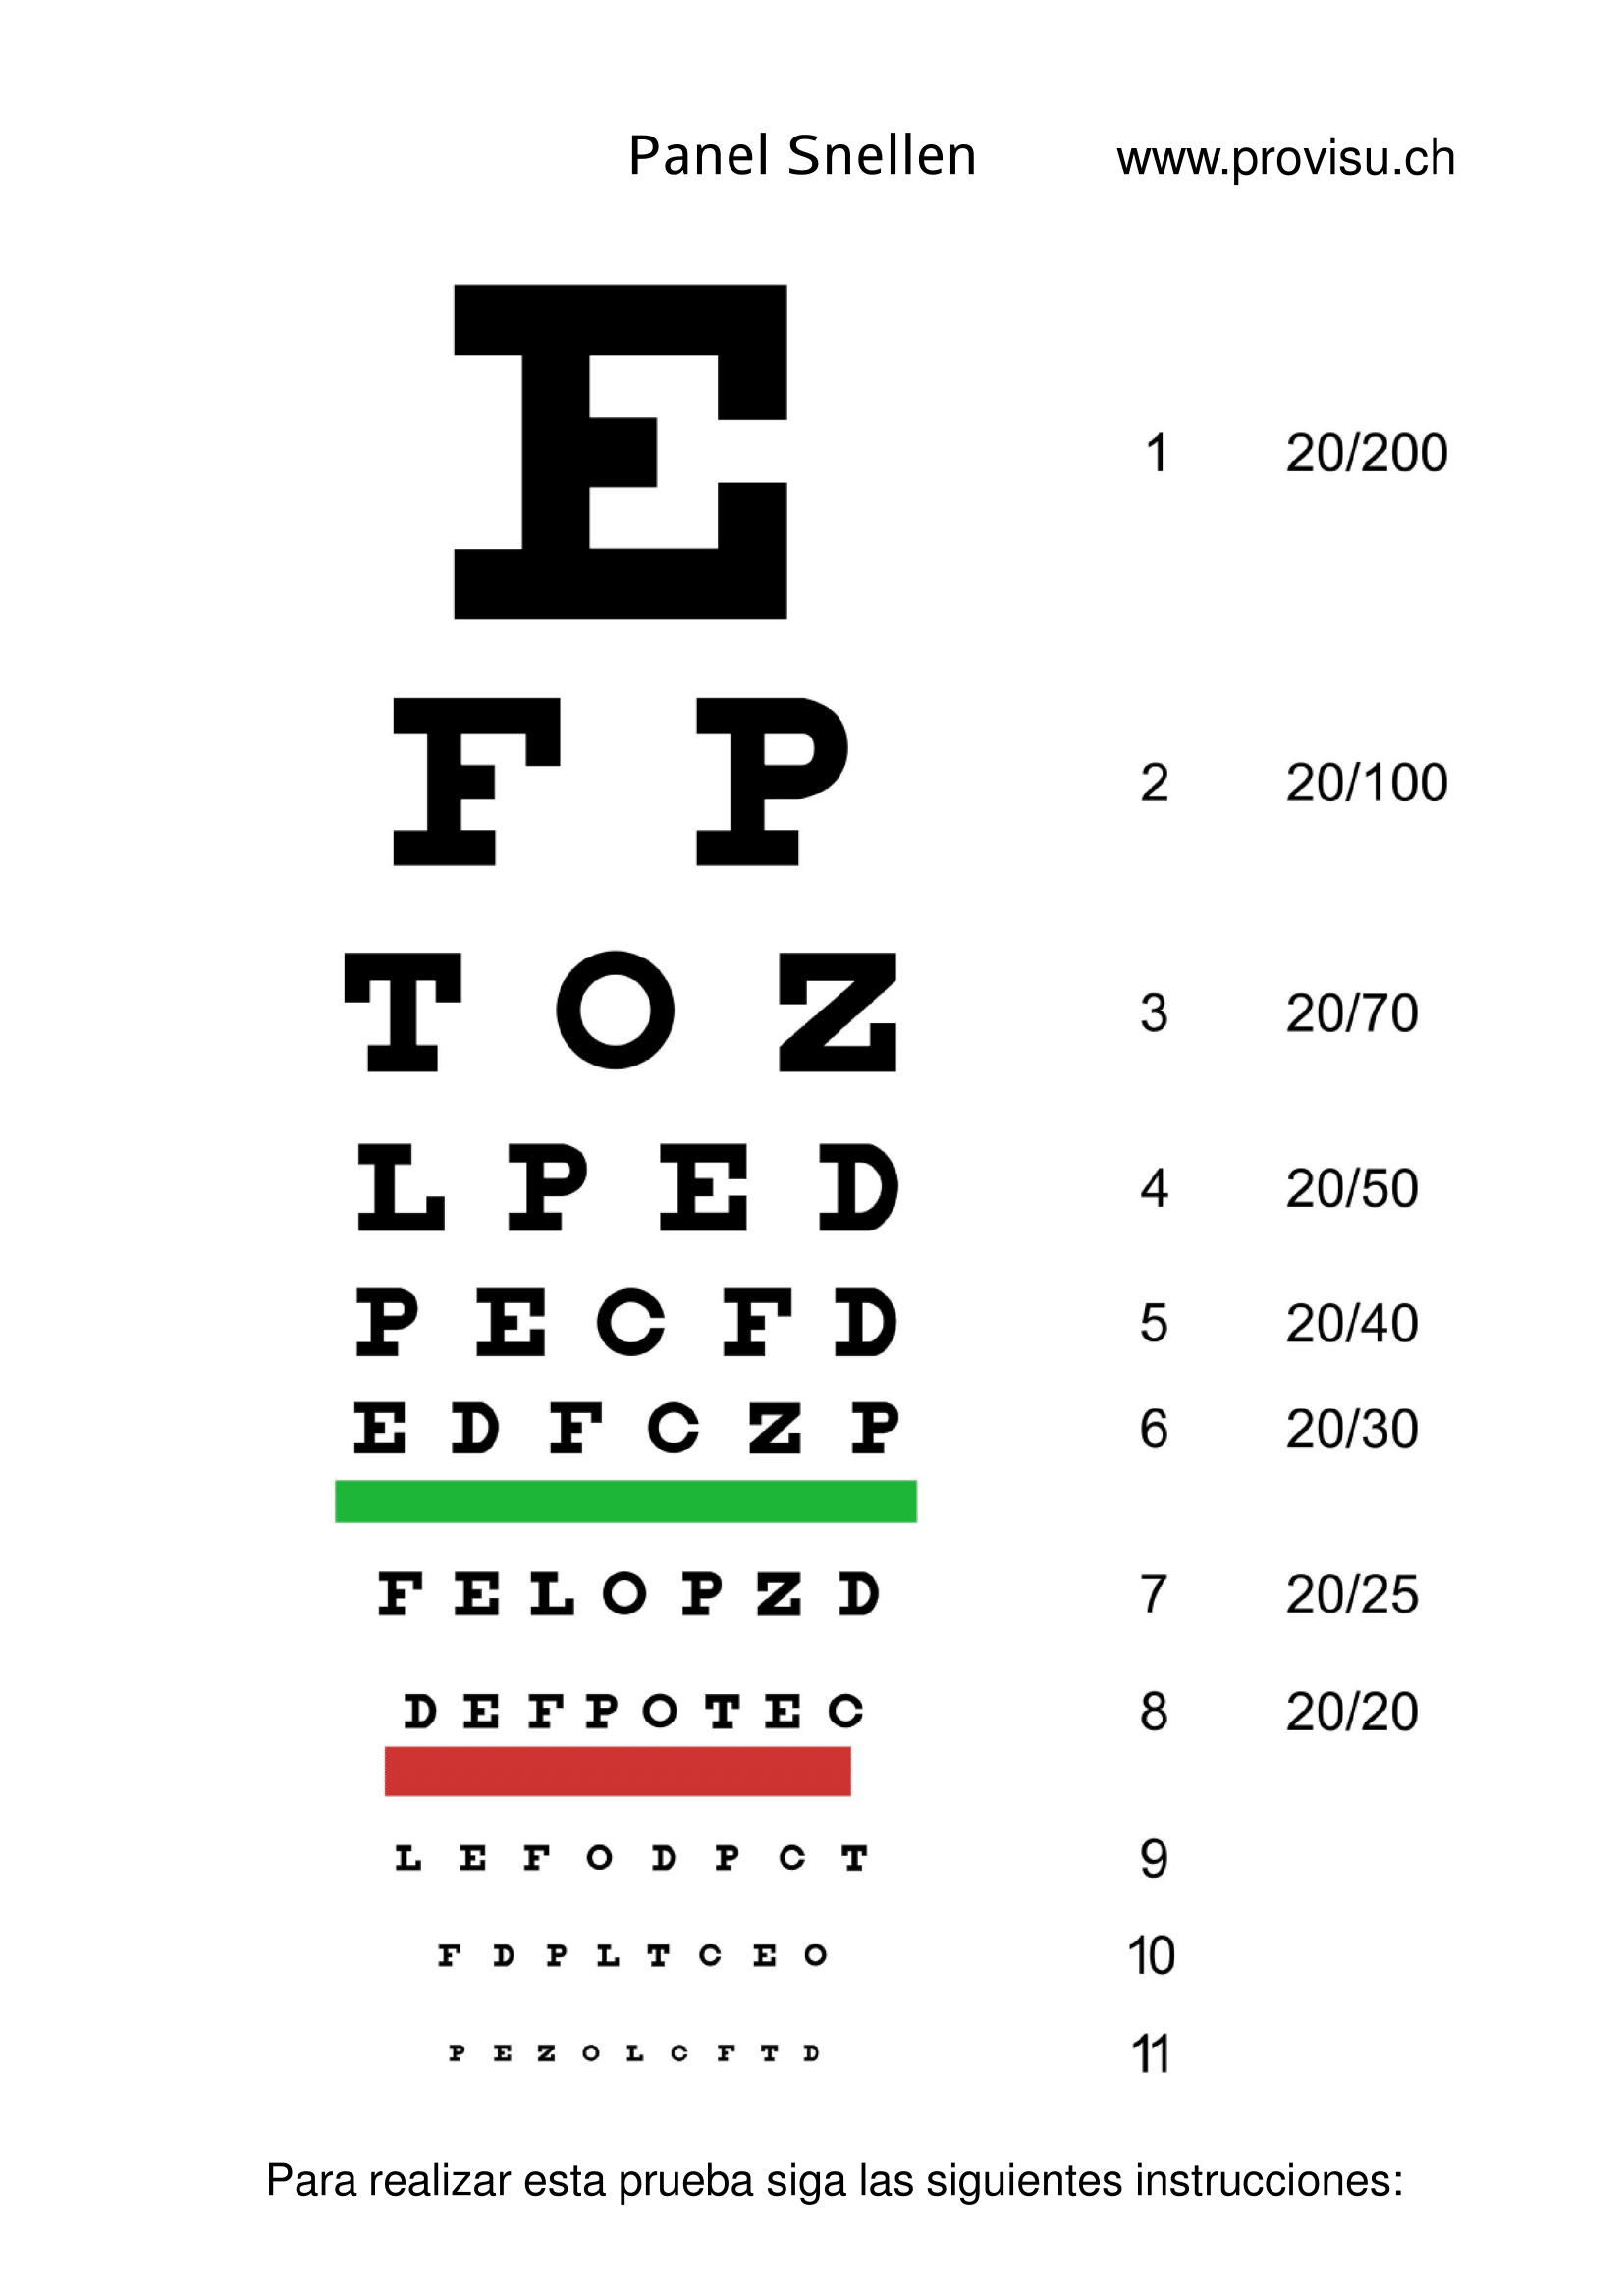
\includegraphics[width=1\linewidth]{img/Snellenchart_es-1.png}
		\caption{Ophthalmological pattern used in the user testing sessions. Source \cite{web:snellen}.}
		\label{fig:add:pattern}
	\end{figure}

	\begin{figure}
		\centering
		\begin{subfigure}[t]{0.5\textwidth}
			\centering
			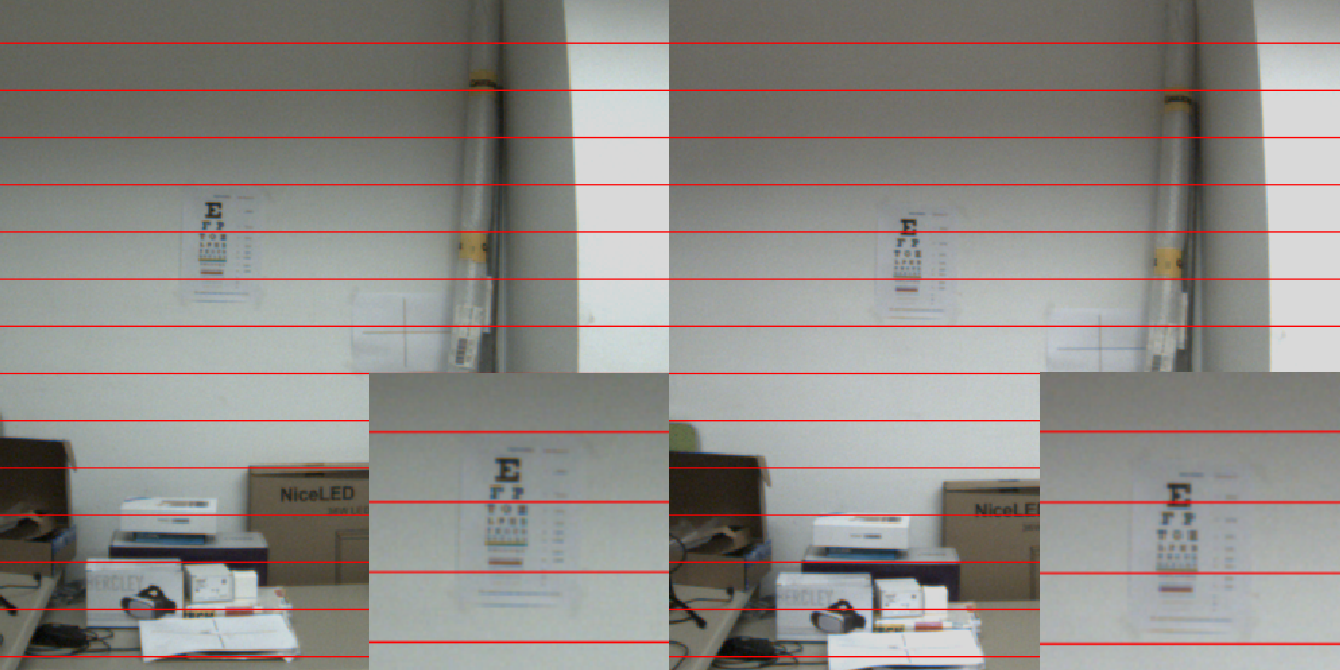
\includegraphics[width=\linewidth]{img/regular2z.png}
			\label{fig:rec:regular}
		\end{subfigure}%
	\vspace{1cm}
		\begin{subfigure}[t]{0.5\textwidth}
			\centering
			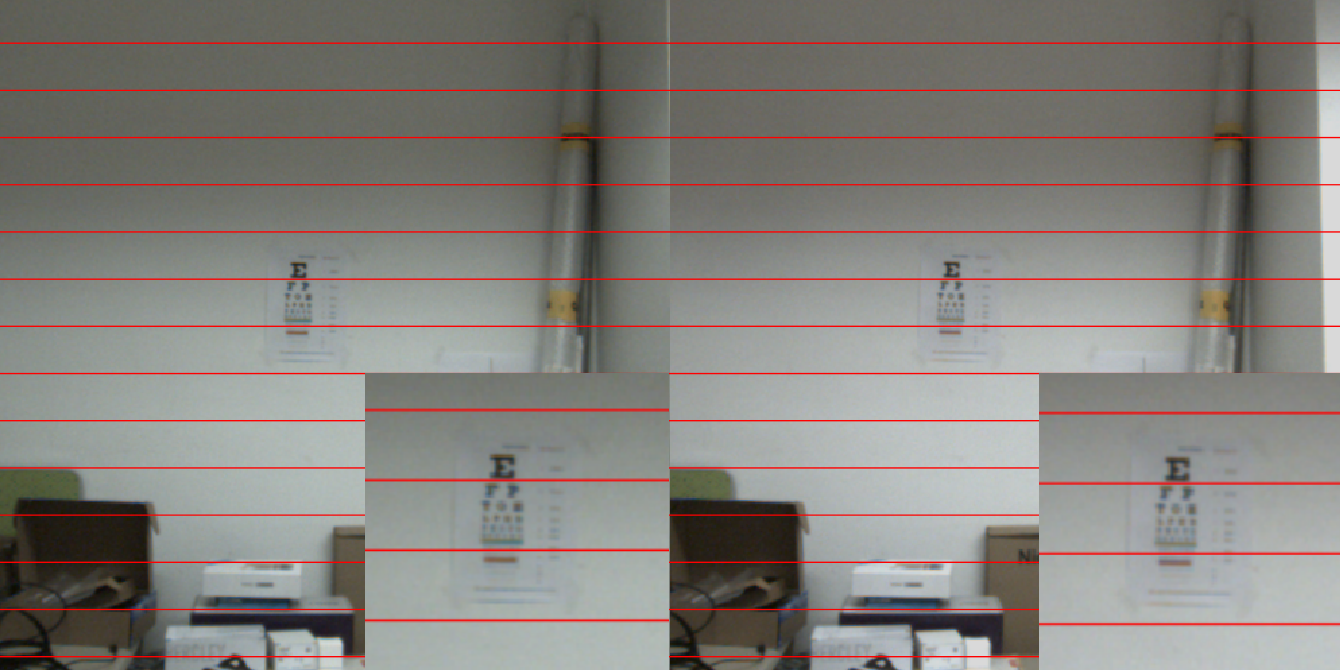
\includegraphics[width=\linewidth]{img/rectified2z.png}
			\label{fig:rec:ractified}
		\end{subfigure}
		\caption{In top there is an example one image pair as it is captured from the cameras, the distortion produced by the optic of the cameras can be noticed. In these images the objects cannot be found on the same Y axis, for example the pattern in the middle of the image. In bottom the same images from the top have been rectified using the calibration module. The distortion, the rotation and the traslation produced by the camera is gone and the objects can be found in the same Y axis. }
		\label{fig:rec}
	\end{figure}
	

\end{document}

